\input{header.tex}
\input{newcommands.tex}

\usetikzlibrary{shapes.gates.logic.US}


\title{Digitale Schaltkreise mit Ti\textit{k}Z erstellen}
\author{Fortbildungsmaterial für MINT-Lehrkräfte}
\date{25. Mai 2025}
\pagestyle{plain}

\begin{document}

\maketitle

Digitale Schaltkreise bilden das Fundament der modernen Computertechnik und sind essentiell für das Verständnis der technischen Informatik. Die visuelle Darstellung von Logikgattern, Schaltungen und deren Verbindungen ist unverzichtbar für die Vermittlung digitaler Grundlagen. Mit Ti\textit{k}Z können MINT-Lehrkräfte professionelle Schaltkreisdiagramme erstellen, die den internationalen Standards entsprechen und komplexe digitale Systeme verständlich visualisieren. Diese Handreichung zeigt, wie Sie von einfachen Gattern bis hin zu komplexen Schaltungen alles mit Ti\textit{k}Z realisieren können.

\section{Grundlagen und benötigte Bibliotheken}

Ti\textit{k}Z bietet mit den \texttt{circuits}-Bibliotheken spezialisierte Funktionen für die Darstellung digitaler Schaltkreise. Diese Bibliotheken stellen vordefinierte Gatter, Verbindungsstile und Layout-Funktionen bereit, die den etablierten Standards der Elektrotechnik und Informatik entsprechen.

Für die Erstellung professioneller Schaltkreisdiagramme benötigen wir mehrere spezialisierte Ti\textit{k}Z-Bibliotheken, die verschiedene Aspekte der digitalen Darstellung abdecken:

\begin{lstlisting}[style=latex]
\usepackage{tikz}
\usetikzlibrary{circuits.logic.US, circuits.logic.IEC,positioning, calc}
\end{lstlisting}

Die \texttt{circuits.logic.US}-Bibliothek stellt amerikanische Gatter-Symbole bereit, wie sie in der US-amerikanischen Norm verwendet werden. Diese rechteckigen Symbole mit charakteristischen Formen sind weit verbreitet und besonders in der Informatik üblich. Die \texttt{circuits.logic.IEC}-Bibliothek bietet europäische Gatter-Symbole nach IEC-Standard mit rechteckigen Grundformen und logischen Symbolen. Die \texttt{positioning}-Bibliothek ermöglicht die intuitive Platzierung von Gattern relativ zueinander, was bei komplexeren Schaltungen unerlässlich ist. Mit \texttt{calc} können wir präzise Verbindungspunkte und Kreuzungen berechnen.



\section{Grundlegende Logikgatter}

Beide Symbolsätze haben ihre Berechtigung: US-Symbole sind intuitiver und visuell unterscheidbarer, während IEC-Symbole kompakter und in Europa standardisiert sind. Wir konzentrieren uns in dieser Handreichung auf US-Symbole, da sie didaktisch vorteilhafter sind.

\subsection{Die wichtigsten Gatter-Typen}

Digitale Schaltkreise bestehen aus verschiedenen Grundgattern, die jeweils spezifische logische Operationen ausführen:

\begin{lstlisting}[style=latex]
\begin{tikzpicture}[circuit logic US]
	% Grundgatter nebeneinander
	\node[and gate] (and1) {};
	\node[or gate, right=2cm of and1] (or1) {};
	\node[not gate, right=2cm of or1] (not1) {};
	\node[nand gate, right=2cm of not1] (nand1) {};
	
	% Beschriftungen
	\node[below=0.3cm of and1] {\small AND};
	\node[below=0.3cm of or1] {\small OR};
	\node[below=0.3cm of not1] {\small NOT};
	\node[below=0.3cm of nand1] {\small NAND};
\end{tikzpicture}
\end{lstlisting}

\begin{ausgabe}
\begin{center}\begin{tikzpicture}[circuit logic US]
% Grundgatter nebeneinander
\node[and gate] (and1) {};
\node[or gate, right=2cm of and1] (or1) {};
\node[not gate, right=2cm of or1] (not1) {};
\node[nand gate, right=2cm of not1] (nand1) {};

% Beschriftungen
\node[below=0.3cm of and1] {\small AND};
\node[below=0.3cm of or1] {\small OR};
\node[below=0.3cm of not1] {\small NOT};
\node[below=0.3cm of nand1] {\small NAND};
\end{tikzpicture}\end{center}
\end{ausgabe}

\subsection{Erweiterte Gatter}

Neben den Grundgattern gibt es weitere wichtige Gatter-Typen:

\begin{lstlisting}[style=latex]
\begin{tikzpicture}[circuit logic US]
	\node[nor gate] (nor1) {};
	\node[xor gate, right=2cm of nor1] (xor1) {};
	\node[xnor gate, right=2cm of xor1] (xnor1) {};
	
	% Beschriftungen
	\node[below=0.3cm of nor1] {\small NOR};
	\node[below=0.3cm of xor1] {\small XOR};
	\node[below=0.3cm of xnor1] {\small XNOR};
\end{tikzpicture}
\end{lstlisting}

\begin{ausgabe}
\begin{center}\begin{tikzpicture}[circuit logic US]
\node[nor gate] (nor1) {};
\node[xor gate, right=2cm of nor1] (xor1) {};
\node[xnor gate, right=2cm of xor1] (xnor1) {};

% Beschriftungen
\node[below=0.3cm of nor1] {\small NOR};
\node[below=0.3cm of xor1] {\small XOR};
\node[below=0.3cm of xnor1] {\small XNOR};
\end{tikzpicture}\end{center}
\end{ausgabe}

\section{Eingänge und Ausgänge}

\subsection{Gatter mit Eingängen}

Logikgatter können verschiedene Anzahlen von Eingängen haben. Ti\textit{k}Z passt die Gatter automatisch an:

\begin{lstlisting}[style=latex]
\begin{tikzpicture}[circuit logic US]
	% 2-Eingang AND-Gatter
	\node[and gate, inputs=nn] (and2) {};
	
	% 3-Eingang AND-Gatter
	\node[and gate, inputs=nnn, right=3cm of and2] (and3) {};
	
	% 4-Eingang OR-Gatter
	\node[or gate, inputs=nnnn, right=3cm of and3] (or4) {};
	
	% Beschriftungen
	\node[below=0.3cm of and2] {\small 2-Eingang};
	\node[below=0.3cm of and3] {\small 3-Eingang};
	\node[below=0.3cm of or4] {\small 4-Eingang};
\end{tikzpicture}
\end{lstlisting}

\begin{ausgabe}
\begin{center}\begin{tikzpicture}[circuit logic US]
% 2-Eingang AND-Gatter
\node[and gate, inputs=nn] (and2) {};

% 3-Eingang AND-Gatter
\node[and gate, inputs=nnn, right=3cm of and2] (and3) {};

% 4-Eingang OR-Gatter
\node[or gate, inputs=nnnn, right=3cm of and3] (or4) {};

% Beschriftungen
\node[below=0.3cm of and2] {\small 2-Eingang};
\node[below=0.3cm of and3] {\small 3-Eingang};
\node[below=0.3cm of or4] {\small 4-Eingang};
\end{tikzpicture}\end{center}
\end{ausgabe}

\subsection{Verbindungen zwischen Gattern}

Gatter werden durch Leitungen verbunden, die über spezifische Anschlüsse verfügen. Wichtig ist dabei eine saubere Leitungsführung ohne Überlappungen:

\begin{lstlisting}[style=latex]
% Praeambel erweitern um:
\usetikzlibrary{shapes.gates.logic.US}

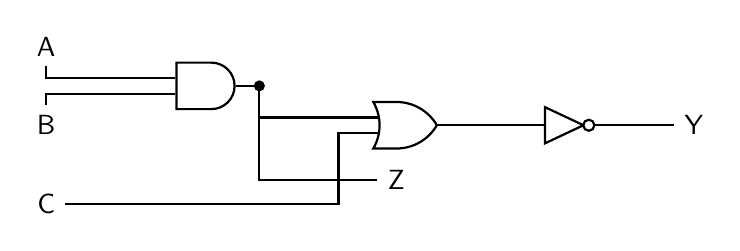
\begin{tikzpicture}[font=\sffamily, thick]
	% Eingangspunkte definieren
	\node (A) at (0, 1) {A};
	\node (B) at (0, 0) {B};
	\node (C) at (0, -1) {C};
	
	% Gatter positionieren
	\node[and gate US, draw, logic gate inputs=nn] at (2, 0.5) (and1) {};
	\node[or gate US, draw, logic gate inputs=nn] at (4.5, 0) (or1) {};
	\node[not gate US, draw] at (6.5, 0) (not1) {};
	
	% Saubere Eingangsleitungen
	\draw (A) |- (and1.input 1);
	\draw (B) |- (and1.input 2);
	\draw (C) -| ([xshift=-0.5cm]or1.input 2) |- (or1.input 2);
	
	% Verbindungen zwischen Gattern
	\draw (and1.output) -- ([xshift=0.3cm]and1.output) |- (or1.input 1);
	\draw (or1.output) -- (not1.input);
	
	% Verknuepfungspunkt fuer Zwischensignal
	\coordinate (junction) at ([xshift=0.3cm]and1.output);
	\draw (junction) |- ++(0,-1.2) -- ++(1.5,0) node[right] {Z};
	\fill (junction) circle (2pt);
	
	% Ausgangsleitung
	\draw (not1.output) -- ++(1,0) node[right] {Y};
	\end{tikzpicture}
	\end{lstlisting}
	
	\begin{ausgabe}
	\begin{center}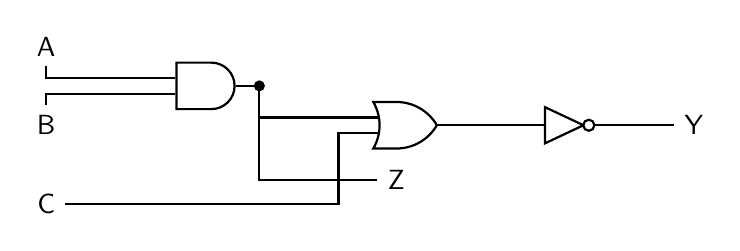
\begin{tikzpicture}[font=\sffamily, thick]
	% Eingangspunkte definieren
	\node (A) at (0, 1) {A};
	\node (B) at (0, 0) {B};
	\node (C) at (0, -1) {C};
	
	% Gatter positionieren
	\node[and gate US, draw, logic gate inputs=nn] at (2, 0.5) (and1) {};
	\node[or gate US, draw, logic gate inputs=nn] at (4.5, 0) (or1) {};
	\node[not gate US, draw] at (6.5, 0) (not1) {};
	
	% Saubere Eingangsleitungen
	\draw (A) |- (and1.input 1);
	\draw (B) |- (and1.input 2);
	\draw (C) -| ([xshift=-0.5cm]or1.input 2) |- (or1.input 2);
	
	% Verbindungen zwischen Gattern
	\draw (and1.output) -- ([xshift=0.3cm]and1.output) |- (or1.input 1);
	\draw (or1.output) -- (not1.input);
	
	% Verknuepfungspunkt fuer Zwischensignal
	\coordinate (junction) at ([xshift=0.3cm]and1.output);
	\draw (junction) |- ++(0,-1.2) -- ++(1.5,0) node[right] {Z};
	\fill (junction) circle (2pt);
	
	% Ausgangsleitung
	\draw (not1.output) -- ++(1,0) node[right] {Y};
\end{tikzpicture}\end{center}
\end{ausgabe}

\subsection{Einfaches Praxisbeispiel: Halbaddierer}

Ein klassisches Beispiel aus der digitalen Technik ist der Halbaddierer, der zwei Bits addiert:

\begin{lstlisting}[style=latex]
\begin{tikzpicture}[circuit logic US, node distance=2cm]
	% Eingangspunkte definieren
	\coordinate (A) at (0,1);
	\coordinate (B) at (0,0);
	
	% Gatter positionieren
	\node[xor gate, inputs=nn] (xor1) at (3,0.5) {};
	\node[and gate, inputs=nn] (and1) at (3,-1) {};
	
	% Eingangsleitungen zu beiden Gattern
	\draw (A) node[left] {A} -- ++(1,0) |- (xor1.input 1);
	\draw (B) node[left] {B} -- ++(1,0) |- (xor1.input 2);
	
	% Gleiche Eingaenge auch zum AND-Gatter
	\draw (A) -- ++(1.5,0) |- (and1.input 1);
	\draw (B) -- ++(1.5,0) |- (and1.input 2);
	
	% Verknuepfungspunkte markieren
	\coordinate (A_branch) at ($ (A) + (1,0) $);
	\coordinate (B_branch) at ($ (B) + (1,0) $);
	\fill (A_branch) circle (1.5pt);
	\fill (B_branch) circle (1.5pt);
	
	% Ausgaenge beschriften
	\draw (xor1.output) -- ++(1,0) node[right] {Summe (S)};
	\draw (and1.output) -- ++(1,0) node[right] {Uebertrag (C)};
\end{tikzpicture}
\end{lstlisting}

\begin{ausgabe}
\begin{center}\begin{tikzpicture}[circuit logic US, node distance=2cm]
% Eingangspunkte definieren
\coordinate (A) at (0,1);
\coordinate (B) at (0,0);

% Gatter positionieren
\node[xor gate, inputs=nn] (xor1) at (3,0.5) {};
\node[and gate, inputs=nn] (and1) at (3,-1) {};

% Eingangsleitungen zu beiden Gattern
\draw (A) node[left] {A} -- ++(1,0) |- (xor1.input 1);
\draw (B) node[left] {B} -- ++(1,0) |- (xor1.input 2);

% Gleiche Eingaenge auch zum AND-Gatter
\draw (A) -- ++(1.5,0) |- (and1.input 1);
\draw (B) -- ++(1.5,0) |- (and1.input 2);

% Verknuepfungspunkte markieren
\coordinate (A_branch) at ($ (A) + (1,0) $);
\coordinate (B_branch) at ($ (B) + (1,0) $);
\fill (A_branch) circle (1.5pt);
\fill (B_branch) circle (1.5pt);

% Ausgaenge beschriften
\draw (xor1.output) -- ++(1,0) node[right] {Summe (S)};
\draw (and1.output) -- ++(1,0) node[right] {Übertrag (C)};
\end{tikzpicture}\end{center}
\end{ausgabe}

\section{Zusammenfassung}

Die Erstellung digitaler Schaltkreise mit Ti\textit{k}Z bietet eine solide Grundlage für die Darstellung der wichtigsten Elemente der digitalen Technik. Die \texttt{circuits.logic}-Bibliotheken stellen professionelle Gatter-Symbole bereit, die internationalen Standards entsprechen und für die Vermittlung digitaler Grundlagen optimal geeignet sind.

Aufgrund der angestrebten Einfachheit dieser Handreichung wurde bewusst auf komplexe Schaltungsbeispiele wie Flip-Flops oder umfangreiche kombinatorische Schaltungen verzichtet. Die hier vorgestellten Grundfunktionen der \texttt{node}-Funktion von Ti\textit{k}Z - wie Positionierung, Verbindungen und Beschriftungen - finden jedoch vollständig Anwendung und lassen sich nahtlos mit den digitalen Gattern kombinieren. Alle bereits erlernten Ti\textit{k}Z-Techniken aus anderen Handreichungen können direkt auf Schaltkreise übertragen werden. Die Kombination aus technischer Präzision und didaktischer Einfachheit macht Ti\textit{k}Z zur idealen Wahl für die Einführung in digitalen Grundlagen der technischen Informatik.

\end{document}